\documentclass{article} % For LaTeX2e
\usepackage{nips15submit_e,times}
\usepackage{hyperref}
\usepackage{url}
\usepackage{graphicx}
\graphicspath{ {images/} }
\usepackage{titlesec}
\titlespacing*{\section}{0pt}{*1}{*0.5}
\titlespacing*{\subsection}{0pt}{*1}{*0.5}
\titlespacing*{\subsubsection}{0pt}{*1}{*0.5}
%\documentstyle[nips14submit_09,times,art10]{article} % For LaTeX 2.09


\title{Identifying Rock, Paper, Scissors Using Neural Networks}


\author{
Andy Sun \\
Department of Witchcraft and Wizardry\\
Simon Fraser University\\
Burnaby, BC V5A 1S6 \\
\texttt{hpsun@sfu.ca} \\
\And
Jacob Patenaude \\
Department of Witchcraft and Wizardry\\
Simon Fraser University\\
Burnaby, BC V5A 1S6 \\
\texttt{jpatenau@sfu.ca} \\
\And
Paul Westlund \\
Department of Witchcraft and Wizardry\\
Simon Fraser University\\
Burnaby, BC V5A 1S6 \\
\texttt{pwestlun@sfu.ca} \\
\And
Wilson Lee \\
Department of Witchcraft and Wizardry\\
Simon Fraser University\\
Burnaby, BC V5A 1S6 \\
\texttt{wla83@sfu.ca} \\
\And
Siddhant Agrawal \\
Department of Witchcraft and Wizardry\\
Simon Fraser University\\
Burnaby, BC V5A 1S6 \\
\texttt{agrawal@sfu.ca} \\
}

% The \author macro works with any number of authors. There are two commands
% used to separate the names and addresses of multiple authors: \And and \AND.
%
% Using \And between authors leaves it to \LaTeX{} to determine where to break
% the lines. Using \AND forces a linebreak at that point. So, if \LaTeX{}
% puts 3 of 4 authors names on the first line, and the last on the second
% line, try using \AND instead of \And before the third author name.

\newcommand{\fix}{\marginpar{FIX}}
\newcommand{\new}{\marginpar{NEW}}

\nipsfinalcopy % Uncomment for camera-ready version

\begin{document}


\maketitle

\begin{abstract}
Recent advances in GPU hardware have resulted in more powerful computational
processing power at extremely low costs. This lowered barrier to entry allows
for neural networks to be trained on modern low-to-mid range PCs. This provides
an efficient and accurate means for classifying even the most niche of datasets,
such as hand gestures in the children's game of Rock-Paper-Scissors. In this
article, we conduct a systematic analysis of the performance of state-of-the-
art computer vision algorithms compared against a pre-trained convolutional
neural network. We also discuss the advantages and drawbacks of both approaches
and note the challenges of both techniques.
\end{abstract}

\section{Introduction}

The game of Rock-Paper-Scissors is simply a problem of classifying images. What we wanted to do was compare the accuracy of a trained neural network to that of a state-of-the-art computer vision algorithm. The difficulty was that we were analyzing a single object (a hand) in different positions rather than different objects. This ruled out the possibility of using algorithms such as colour histograms which use an object's colour for classification. One computer vision algorithm which has had much success in object recognition is Scale Invariant Feature Transform (SIFT) \cite{SIFT}. This algorithm uses keypoints -- defining features of an object -- to identify objects. SIFT does well at classifying objects even when they are rotated or scaled slightly. The neural network we used is a derivative of the InceptionV3 network; a network which can distinguish between a thousand different categories with accuracies rivalling humans' abilities. We compared these two approaches of object recognition to find out if a neural network is comparable to a state-of-the-art computer vision algorithm. We looked at both accuracy as well as how fast each method can run on a mid range computer. We also looked at the viability of using these methods to run on a live video feed.

\subsection{Collecting Images}
Both methods needed images of hands in the positions of Rock, Paper, and Scissors to learn what each looks like. We began by imaging many different peoples' hands in these three positions. The hands were in various orientations (towards the camera, sideways, etc.) and the images were taken in different locations so there would be variations in background and lighting.  We also tried to have a good representation of hand size, skin colour, wrinkles, and hair to ensure that our algorithms would work on most hands. We captured 430 images in total with about 140 images for each of the three positions using a simple laptop webcam. The neural network we decided to use required images which were 299$\times$299, so we cropped each of our images to this size. We then randomly split our images into a training set and a validation set with about the same number of images in each. This data was used by both the neural network and SIFT to ensure any differences in their performance were not a result of the data.

\begin{figure}[h]
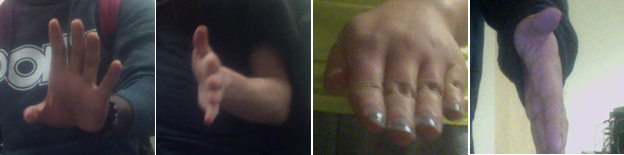
\includegraphics[scale=0.8]{paper_image_nn.png}
\centering
\caption{Training images of various paper hand gestures}
\end{figure}

\begin{figure}[h]
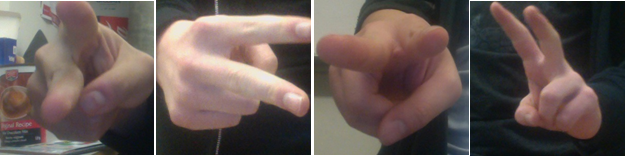
\includegraphics[scale=0.8]{scissors_image_nn.png}
\centering
\caption{Training images of various scissor hand gestures}
\end{figure}

\begin{figure}[h]
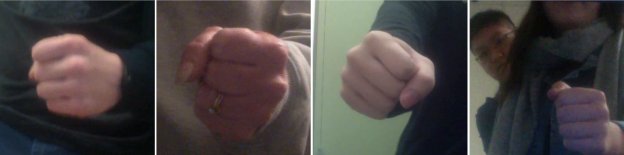
\includegraphics[scale=0.8]{rock_image_nn.png}
\centering
\caption{Training images of various rock hand gestures}
\end{figure}

\subsection{Hand Tracking}
Because we wanted to asses the possibility of these methods being used on a live video feed, we needed a method to automatically crop the 1280$\times$720 images down to 299$\times$299 images while containing as much of the hand as possible. Since this is just a problem of hand tracking, we decided to use a computer vision algorithm called colour indexing \cite{swain}. This method uses a model of the object to be tracked and records the colour distribution of that model -- its colour histogram. Then, for each image to be analyzed, the likelihood of each of its pixel being part of the model is calculated using the model histogram; this produces a probability image. Finally, we use mean shift to find the most likely location of the hand. The benefit of this method is it is fast and can track a hand regardless of what position the hand is in. One drawback of this method is, since it is basically looking for skin colours, it can easily end up tracking the user's head instead of their hand. To address this, we decided that the camera should face the user's chest so their head is above the top of the view. This reduced the issue, however it still has trouble locating just the hand when the user also has their arm exposed. We used three images of hand as our models and were easily able to track a hand in realtime. 

\section{SIFT Approach}
\label{sift}

Lowe's algorithm generates a set of keypoints along with keypoint descriptors.  These keypoints are selected by detecting areas of high curvature and contrast at all scales (Figure~\ref{sift_scales}), and then refined based on keypoint stability. The corresponding descriptors are then generated by calculating the gradient of the region, realigning the gradients to the largest relative gradient to provide local rotational invariance, and transforming the local gradients into a 128 bin feature vector (Figure~\ref{sift_kp_gradient}). The resulting array is resistant to changes in illumination and image distortion.

\begin{figure}[h]
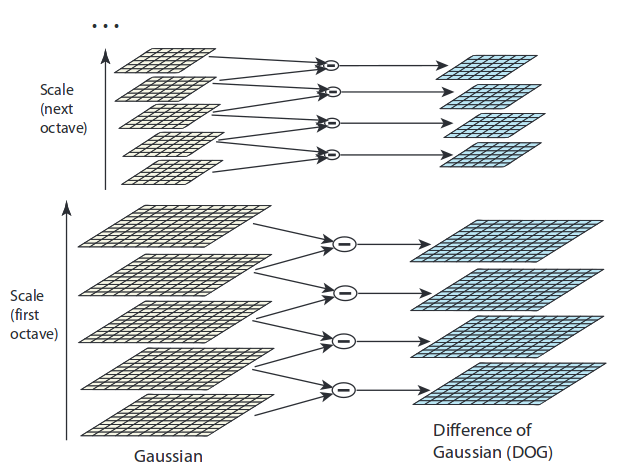
\includegraphics[scale=0.3]{dog_pyramid.png}
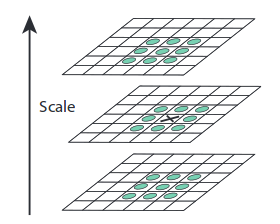
\includegraphics[scale=0.6]{pyramid_extrema.png}
\centering
\caption{Taken from Lowe \cite{SIFT}, an difference-of-Gaussian image pyramid is constructed to estimate the Laplacian at each level. At each pixel location, its neighbouring 26 pixels are checked for scale-space extrema as keypoint candidates.}
\label{sift_scales}
\end{figure}

These descriptors can then be used to match two keypoints together by comparing the Euclidean distance between any two pairs of keypoints. In his paper, Lowe suggests a method of 2-nearest neighbours matching where a correct match is determined by taking the ratio of the distance of the closest and the second closest matches. He proposes a ratio of 0.75 to be optimal, and in our testing we have found this to be accurate on our dataset of 215 training and 196 validation images (See Table~\ref{sift_ratios}). Due to the small size of this dataset, we opted to store our keypoints in-memory in an array and perform a brute-force match on all training data as opposed to storing in a k-d tree.

\begin{figure}[h]
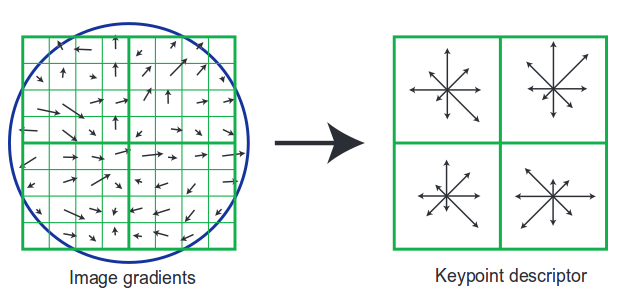
\includegraphics[scale=0.6]{keypoint_orientation.png}
\centering
\caption{Taken from Lowe \cite{SIFT}, the gradients of the keypoint region are divided into smaller windows. At each window, the gradients are rotated to align to the dominant gradient.}
\label{sift_kp_gradient}
\end{figure}

SIFT has a large limitation due to only working in one-dimensional color space, and consequently images need to be either converted to grayscale or run on only one color basis vector. By converting into grayscale, color-based depth and contrast information is lost and by extension, possible keypoint candidate locations. However, using only one color basis vector results in a similar predicament as the additional information encoded is not fully utilized. One possible workaround is to convert into HSV color space and to apply SIFT on the hue basis vector, as it retains color data at the cost of ``colorfulness." However, the drawback is that it takes a significant amount of time to convert from RGB color space to HSV, which detracts from our goal of a real-time gesture classifier.

\begin{figure}[h]
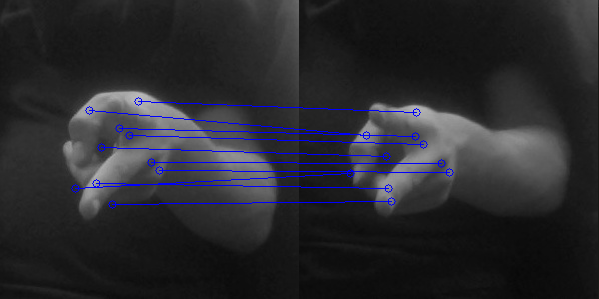
\includegraphics[scale=0.6]{kp_matching_left_test_right_train.png}
\centering
\caption{Visualization of matched SIFT keypoints. The image on the left is from the validation set, while the image on the right is from the training set.}
\label{sift_kp_matching}
\end{figure}

\section{Neural Network Approach}
\label{neural_network}
Our approach for building our convolutional neural network is to start with a baseline network to see what the results we can get from the start. From then on we can branch out and tweak with different network structures and hyper parameters to see how far we can fine tune and improve it to get better results.
We will base our approach by using the pre-trained Inception V3 network as the base for what we will build upon in a technique called transfer learning. This allows us to take advantage of an already fully trained powerful classification model that we can use to retrain for a new set of classes. By doing this, we can get pretty decent results out of the box this way which will cut down on the amount of work needed to train a completely new network from scratch as there isn’t enough time or data available. We will be using this pre-trained network in order to extract features for the 3 new Rock, Paper, Scissors classes which will help in classifying them. We will also be fine tuning the weights of the pre-trained network by retraining some of the later layers in the network in order to conform to our dataset as these later layers may contain weights specific to the ImageNet classes.

\begin{figure}[h]
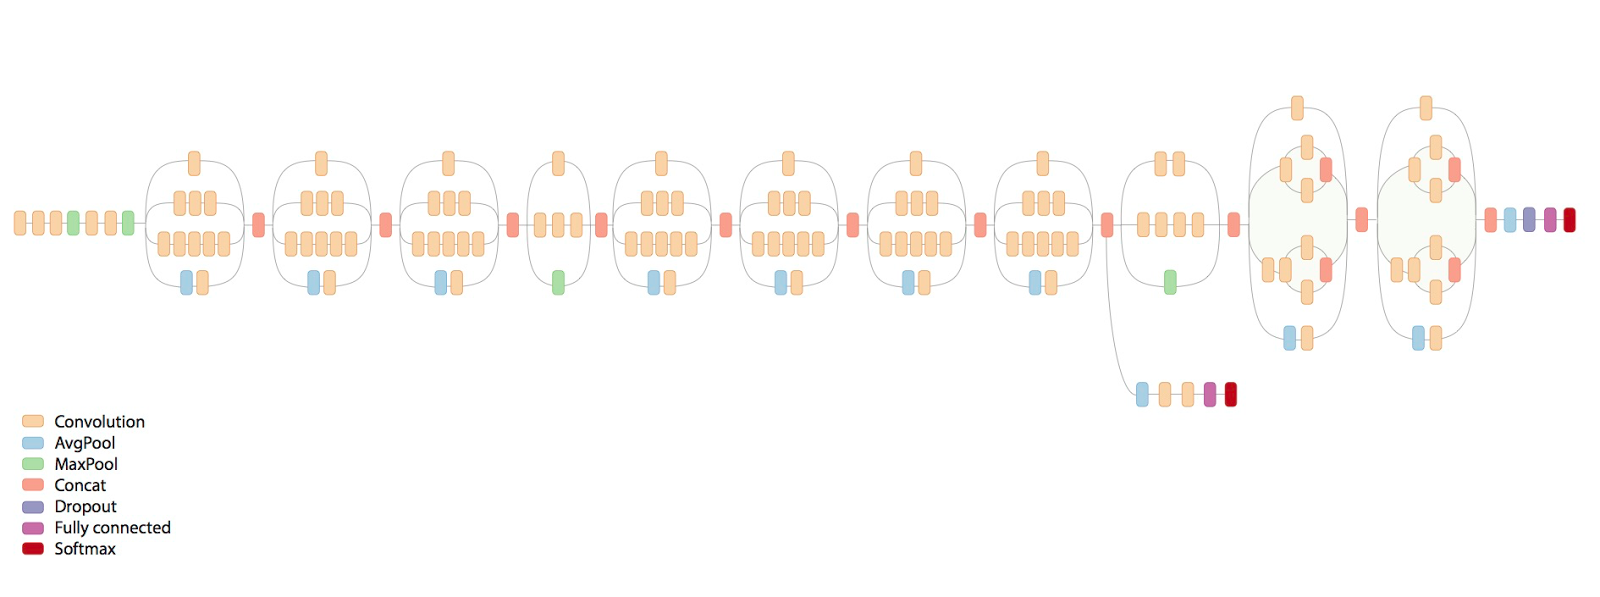
\includegraphics[scale=0.3]{nn_pic.png}
\centering
\caption{The original inception V3 network structure}
\end{figure}

Each network we produce will be trained for 300 epochs using all 215 training and 196 validation images per epoch. Each network can then be benchmarked to see if improvements were made in terms of accuracy and validation accuracy and we can choose the one with the best results are our network of choice.
\subsection{Experiments}

For our neural network, we will experiment with differing network structures and hyperparameters while iterating to see which one performs the best.
\subsubsection{Baseline}
This network was our starting point and is quite simple. It takes the Inception V3 model and replaces the last dense layer with 3 more layers, a 32 node fully connected layer, a dropout layer and finally the output layer (with 3 output nodes for our classes). The output layer uses the softmax activation whereas the fully connected layer uses ReLU. This network was trained with the loss function set to categorical cross entropy and the optimizer set to stochastic gradient descent (with a learning rate of 0.01).

Results: Accuracy – 98\%, Validation Accuracy – 78\%

With this baseline network, it seems that our validation accuracy is not that great. The way to go and improve that is to use regularization to reduce overfitting. The simple way to do this is with dropout layers which sets a fraction of the input units to 0 at each update during training. Our baseline network already includes a single dropout layer before the classification layer, but it did not look like it was enough.
\subsubsection{Network 1}

Network1 consisted of replacing the top classification layer of Inception V3 and adding a GlobalAveragePooling2D layer, 32 node fully connected layer, a dropout layer, and finally the output layer. This time, the dropout was increased to 0.8 to see if that will improve our validation accuracy. For training, the layers that we added were trained first using rmsprop as the optimizer while everything else was frozen, then the last two blocks of Inception V3 were unfrozen and the network was trained again. This time for stochastic gradient descent, we went with a learning rate of 0.0001 and momentum of 0.9.

Results: Accuracy – 92\%, Validation Accuracy – 78\%

This time, the accuracy went down but the validation accuracy didn’t improve.
\subsubsection{Network 2}

For network2, we simply tried training all the layers from network1 in one go.

Results: Accuracy – 92\%, Validation Accuracy – 73\%

This made things worse as the accuracy was the same but the validation accuracy dropped down to around 73%.
\subsubsection{Network 3}

For network3, we decided to add another dropout layer onto network2 after the GlobalAveragePooling2D layer with it set at 0.5, just to see if it helps anymore with overfitting. 

Results: Accuracy – 99\%, Validation Accuracy – 78\%

The results were that the accuracy surprisingly went up for both, this seemed more promising.
\subsubsection{Network 4}

We saw from network3 that adding another dropout layer made our validation accuracy better, so why not do it again. For network4 we added another dropout layer to just before the GlobalAveragePooling2D layer, also with it set to 0.5. 

Results: Accuracy – 99\%, Validation Accuracy – 80\%

This time, the accuracy was still at 99\% but the validation accuracy improved again to around 80\%, so things are improving slowly.
\subsubsection{Network 5}

For network5, we took network4 but trained it in two steps like in network 1 – the layers that we added were trained first using rmsprop as the optimizer while everything else was frozen, then the last two blocks of Inception V3 were unfrozen and the network trained again. 

Results: Accuracy – 99\%, Validation Accuracy – 77\%

The accuracy remained at 99\% but validation accuracy dropped to around 77\%, which is not any better.
\subsubsection{Network 6}

From network5, it looked like the validation accuracy was oscillating quite a bit around the 77\% range, so for network6 we set the stochastic gradient descent parameters to have a momentum of 0 and a learning rate of 0.01.

Results: Accuracy – 100\%, Validation Accuracy – 84\%

This proved to be the most promising so far as accuracy went to 100\% and validation accuracy went to 84\%, which is the best so far.
\subsubsection{Network 7}

From what we learned from network6 is that our validation accuracy varied a lot depending on our stochastic gradient descent parameters. It seems like we may be stuck at some local minima in our loss function. For network7 we removed the dropout layer just before the GlobalAveragePooling2D layer. This time we tweaked with the hyperparameters even more, setting the learning rate to 0.01, learning rate decay to 1e-6 and momentum to 0.9

Results: Accuracy – 100\%, Validation Accuracy – 90\%

This proved to give the best results that we could get with accuracy of 100\% and validation accuracy of 90\%, which is a huge improvement over network6.
\subsubsection{Network 8}

This network just added back the dropout layer that was removed in network7.

Results: Accuracy – 100\%, Validation Accuracy – 85\%

The results were similar, but the validation accuracy oscillated a lot between 82-90\%.
\subsection{Observations}
During training, we found out that 300 epochs was usually where the training and validation accuracy would plateau. Beyond that point, the results did not improve significantly. This is probably due to the fact that dataset was simply too small. If we had a lot more data, then our results may have improved some more.
We also noticed that when our network classified an image wrong, it was usually totally off. For example, the classification score for an image would be 0.99 for Paper when it was actually Scissors. This was the case for a lot of the images that it got wrong. It would be quite certain that an image is of one class, but be off completely. This is most likely due to overfitting as our dataset did not have enough varying examples.


\section{Performance}
\label{performance}

In this section, we discuss the real-world performance obtained by running the SIFT detection algorithm as described in section~\ref{sift} and the neural network as described in section~\ref{neural_network}. We chose a relatively old, mid-range laptop to run the tests on as it was the machine that we intended to use for our demo during the poster session. The laptop was a 2012 Macbook equipped with a 2.9 GHz dual core Intel Core i7, 8 GB RAM, Intel HD Graphics 4000, running on macOS Sierra 10.12.1.

\subsection{SIFT}

\begin{table}[t]
\caption{SIFT Ratios Matches}
\label{sift_ratios}
\begin{center}
\begin{tabular}{ll}
\multicolumn{1}{c}{\bf RATIO}  &\multicolumn{1}{c}{\bf INCORRECT MATCHES}
\\ \hline \\
0.50             &111 of 196 \\
0.60             &105 of 196 \\
0.70             &100 of 196 \\
0.72             &95 of 196 \\
0.74             &95 of 196 \\
0.76             &91 of 196 \\
0.78             &94 of 196 \\
0.80             &98 of 196 \\
0.90             &102 of 196 \\
\end{tabular}
\end{center}
\end{table}

[WIP] The SIFT gesture detector was able to run in real-time, although it only had an accuracy of 53.57\%.

\subsection{Neural Network}
Out of all the networks, network7 performed the best with 100\% training accuracy and 90\% test accuracy.

\begin{figure}[h]
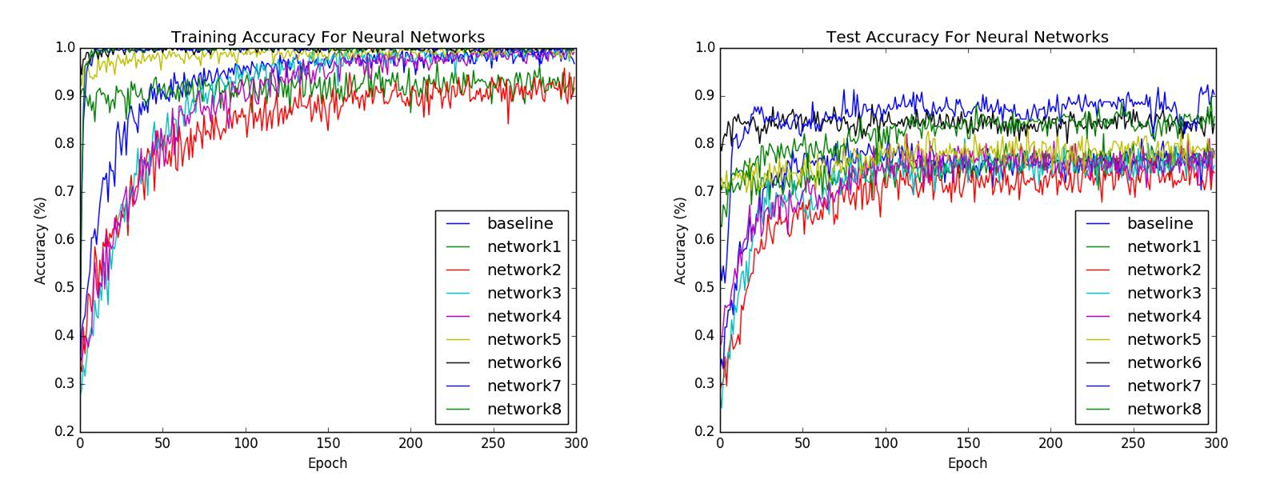
\includegraphics[scale=0.35]{accuracy.png}
\centering
\caption{Training and test accuracy of all the neural networks}
\end{figure}

\section{Conclusion}

Do not change any aspects of the formatting parameters in the style files.
In particular, do not modify the width or length of the rectangle the text
should fit into, and do not change font sizes (except perhaps in the
\textbf{References} section; see below). Please note that pages should be
numbered.

\section{Contributions}

\subsubsection*{Andy Sun}
\begin{itemize}
\item Bullet \#1
\item Bullet \#2
\end{itemize}

\subsubsection*{Jacob Patenaude}
\begin{itemize}
\item Bullet \#1
\item Bullet \#2
\end{itemize}

\subsubsection*{Paul Westlund}
\begin{itemize}
\item Bullet \#1
\item Bullet \#2
\end{itemize}

\subsubsection*{Wilson Lee}
\begin{itemize}
\item Neural Network
\item Rock, Paper, Scissors Game Demo
\end{itemize}

\subsubsection*{Siddhant Agrawal}
\begin{itemize}
\item Poster
\item Report
\end{itemize}


\subsubsection*{References}

References follow the acknowledgments. Use unnumbered third level heading for
the references. Any choice of citation style is acceptable as long as you are
consistent. It is permissible to reduce the font size to `small' (9-point) 
when listing the references. {\bf Remember that this year you can use
a ninth page as long as it contains \emph{only} cited references.}

\begin{thebibliography}{99}
\bibitem{SIFT} Lowe, D. G., ``Distinctive Image Features from Scale-Invariant Keypoints'', \textit{International Journal of Computer Vision} 60:2, 91--110 (2004).
\bibitem{swain} Swain, M. J. and Ballard, D. H., ``Color Indexing''. \textit{International Journal of Computer Vision} 7:1, 11--32 (1991).
\end{thebibliography}

\end{document}
